\documentclass[a4paper, 10pt, onecolumn]{article}

%% Layout related
\usepackage{hyperref}
\usepackage{lscape}

%% Encode
\usepackage[utf8]{inputenc}

%% Graphic related
\usepackage{xcolor}
\usepackage{graphicx}
\graphicspath{{include/img/}}
\DeclareGraphicsExtensions{.jpeg,.jpg,.png}

%% Listing related
\usepackage{enumerate}
\usepackage{paralist} %% enumerate several elements on a single line like (i)
                      %% this is an example, (ii) this is a second example
\newcommand{\benumline}{\begin{inparaenum}[\itshape i\upshape)]}
\newcommand{\eenumline}{\end{inparaenum}}
\usepackage{listings}
%% All the code below is from
%% https://en.wikibooks.org/wiki/LaTeX/Source_Code_Listings
\definecolor{mygreen}{rgb}{0,0.6,0}
\definecolor{mygray}{rgb}{0.5,0.5,0.5}
\definecolor{mymauve}{rgb}{0.58,0,0.82}
\definecolor{lightgray}{gray}{0.9}
\lstset{ %
  backgroundcolor=\color{white},
  basicstyle=\footnotesize\ttfamily,     
  belowcaptionskip=1\baselineskip,
  breakatwhitespace=false,      
  breaklines=true,              
  captionpos=b,                 
  commentstyle=\color{mygreen}, 
  extendedchars=true,           
  frame=single, 
  keepspaces=true,
  keywordstyle=\color{blue},    
  language=C,                   
  %numbers=none,                 
  numbersep=5pt,                
  numberstyle=\tiny\color{mygray},
  rulecolor=\color{black},        
  showspaces=false,               
  showstringspaces=false,         
  showtabs=false,                 
  stepnumber=2,                   
  stringstyle=\color{mymauve},    
  tabsize=4,
  title=\lstname
  xleftmargin=\parindent,
}

\lstdefinestyle{almos}{
  backgroundcolor=\color{lightgray},
  keywordstyle=\bfseries\color{mygreen},
  commentstyle=\itshape\color{mymauve},
  identifierstyle=\color{black},
  stringstyle=\color{orange},
  morekeywords={pid_t, uid_t, gid_t,
    uint_t, uint16_t, uint32_t, uint64_t, spinlock_t, mcs_lock_t, atomic_t,
    bool_t, error_t, task_s, thread_s, cluster_s, cpu_s, list_entry, page_s,
    sig_mgr_s, event_s, rwlock_s, vmm_s, pmm_s, vfs_node_s, vfs_file_s,
    fd_info_s, metafs_s, wait_queue_s, mapper_s, vfs_stat_s, vfs_context_s,
    vfs_node_s, vfs_file_s, vfs_node_op_s}, }

%% Shortcuts
\newcommand{\todo}[1]{\textbf{\color{red}#1\newline}}

%% Firt page related
\author{Pierre-Yves Péneau} \date{\today} \title{Processus, fork() et exec() sur le noyau ALMOS}

\begin{document}

	\maketitle
	\tableofcontents
	  
  \chapter{Introduction}

  \hspace{1cm}Au milieu des années 2000, les fabricants de processeurs ont
  atteint une limite technique.  Au-delà de 100 Watts par boitier, il est
  difficile de refroidir les circuits à l'aide de simples ventilateurs. Les
  technologies comme le water cooling~\citep{googleXXXXdatacenters} sont
  coûteuses et énergivores.  Pour continuer l'augmentation de puissance des
  processeurs en profitant de la loi de Moore, ils ont dû cesser de complexifier
  l'architecture des c\oe urs et d'augmenter leur fréquence de
  fonctionnement. Au contraire, ils ont simplifié les c\oe urs pour en mettre
  plusieurs par processeur.  De nos jours, les architectures à 8 c\oe urs sont
  courantes, celles à une cinquantaine de c\oe urs sont disponibles, et d'autres
  comportant plusieurs centaines, voire milliers, sont à prévoir.
  L'augmentation du nombre de c\oe urs par processeur permet l'augmentation du
  nombre d'instructions exécutées par cycle.  Cela impose une augmentation de la
  quantité de mémoire nécessaire et du débit des accès~\citep{hp2012z820,
    puget2013z9pe}. Les systèmes d'exploitation doivent s'adapter pour gérer
  efficacement ces nouvelles ressources.\\

  \hspace{1cm}Dans ce stage, l'architecture matérielle considérée est
  l'architecture TSAR~\citep{greiner2009tsar} développée au LIP6. TSAR est une
  architecture NUMA (\textit{Non Uniform Memory Acces}) à mémoire partagée
  cohérente, composée de 1024 c\oe urs 32 bits et 1To de mémoire physique (40
  bits).  Les c\oe urs sont répartis en clusters contenant chacun 4 c\oe urs et
  gérant un segment de 4Go de mémoire physique. Le choix de c\oe urs 32 bits, et
  non 64bits, est assumé. C'est, selon les architectes, le meilleur compromis en
  énergie dissipée par instruction et cela permet un meilleur usage des caches
  car les pointeurs sont plus petits.  Un système d'exploitation nommé
  ALMOS~\citep{almaless2011almos} a été spécialement développé pour TSAR. Ce
  système est basé sur un noyau monolithique, tout comme Linux ou *BSD. ALMOS
  signifie \textit{Advanced Locality Management Operating System}. En effet, son
  but premier est le placement efficace des données dans les segments mémoires,
  et des threads accédant à ces données sur les c\oe urs.\\

  \hspace{1cm}L'architecture TSAR utilisée lors du développement d'ALMOS n'était
  pas finalisée. Elle ne proposait que 4Go de mémoire physique (32 bits). Elle
  gère désormais 1To (40 bits). Le but de ce stage est de faire évoluer ALMOS
  pour permettre la gestion de ce tera octet.\\

  \hspace{1cm}Nous faisons face à plusieurs problèmes. Le premier est que les
  c\oe urs 32 bits sont limités à 4Go d'espace adressable virtuel. Le noyau doit
  gérer un espace mémoire physique supérieur à l'espace virtuel des
  processeurs. Pour résoudre ce problème, nous verrons que nous allons devoir
  répartir et souvent répliquer toutes les structures du noyau dans chaque
  cluster. \todo{ALMOS, dans sa version 32 bits, a déjà une organisation
    clusterisée pour gérer le co-placement des threads et des données, mais cela
    n'interdit pas d'accéder facilement à toute la mémoire, c'est désormais
    difficile.} Le deuxième problème est donc de revoir la répartition ou
  réplication des structures du noyau et leur mode d'accès. ALMOS va ainsi
  évoluer vers une structure semblable par certains aspects au
  multi-noyau~\citep{baumann2009multikernel}. Ainsi, le troisième problème est
  une conséquence du deuxième. Si certaines structures sont répliquées, il faut
  que le système en garantisse la cohérence et ainsi offre à l'utilisateur
  l'illusion d'un noyau monolithique. \\

  \hspace{1cm}Pour ce stage, nous allons nous concentrer sur les structures
  partagées par les threads d'un processus, telles que les descripteurs de
  fichiers ou les zones mémoires partagées. \\


  \hspace{1cm}Ce document est organisé de la manière suivante: dans le
  chapitre~\ref{chap:subject}, nous présenterons le sujet du stage et la
  problématique. Le chapitre~\ref{chap:sol} expliquera la solution envisagée
  pour ce répondre à la problématique. Ensuite, nous donnerons dans le
  chapitre~\ref{chap:tasks} le découpage des tâches identifié. Enfin, nous
  donnerons dans le chapitre~\ref{chap:tests} la procédure de recette qui sera
  utilisée pour valider notre solution, et dans le chapitre~\ref{chap:sched}
  l'échéancier retenu pour ce travail.

  \section{La structure task} \label{sec:task}

La structure \texttt{task} (donnée en annexe) est l'abstraction permettant de
définir la notion de \textbf{processus}. Elle porte le même nom dans ALMOS que
dans Linux, et l'équivalent *BSD est la \texttt{struct proc}.  Voici la liste
non exhausitves de toutes les structures contenues ou pointées (la différence
est importante) par la \texttt{struct task}:

  \begin{enumerate}[-]

    \item \texttt{struct task} : le processus doit connaitre son père
        
    \item \texttt{struct cluster\_s} : la structure représentant le cluster sur
      lequel est le processus
    
    \item \texttt{struct cpu\_s} : la structure représentant le cpu sur lequel
      est le processus\footnote{Cette variable serait à supprimer, puisqu'on
      peut avoir l'information via la structure \texttt{cluster\_s}}

    \item \texttt{struct vmm\_s} : le gestionnaire de mémoire virtuel.  Cette
      structure est \textbf{contenue} dans la \texttt{struct task}, \emph{i.e.}
      il n'y a \textbf{pas de pointeurs}

    \item \texttt{struct vfs\_node\_s} : la structure du VFS représentant un
      noeud dans l'arborescence. Ici, le processus connait le noeud racine
      (\textbf{/}) et le répertoire de travail courant

    \item \texttt{struct fd\_info\_s} : cette structure représente les
      descripteurs de fichiers ouverts. On y trouve également la \textbf{table
      de pages}. De même que pour le gestionnaire de mémoire virtuelle, la
      structure \texttt{fd\_info\_s} est \textbf{contenue} par la \texttt{struct
      task}
          
    \item \texttt{struct thread\_s} : cette structure contient tous les threads
      de ce processus.

  \end{enumerate}

  Un processus est donc un ensemble de données permettant de l'identifier
  (\texttt{pid, ppid}), ainsi qu'un ensemble de structures qu'il manipule lors
  de son exécution. Nous allons maintenant nous intéresser à ces structures. On
  donnera le contenu de ces structures de manière non détaillée, en insistant
  sur les points importants.


  \subsection{Les clusters et les processeurs}

    La structure \texttt{cluste\_s} permet une représentation abstraite des
    clusters physique réels de la machine. Un cluster est composé principalement
    des gestionnaires de mémoires, de caches, du tas. On trouve également les
    threads noyaux et les processeurs du cluster.

    Les processeurs sont eux représentés par la structure \texttt{struct
    cpu\_s}.  Ils contiennent l'ordonnanceur, le gestionnaire d'interruption et
    les gestionnaires d'évènements (locaux et distants).

  \subsection{Le gestionnaire de mémoire virtuelle}

    Cette structure est une des plus importante du noyau. C'est elle qui offre
    la vue de la mémoire virtuelle, permettant à chaque processus d'avoir son
    espace d'adressage contigüe (virtuellement), et de penser qu'il est le seul
    sur la machine. Cette structure utilise un gestionnaire de mémoire physique
    (la \texttt{struct pmm\_s}), et pointe également sur une autre structure (la
    \texttt{struct vm\_region\_s} contenant les fonctions relatives à cette
    mémoire virtuelle (\texttt{page\_swap\_in/out()}, \texttt{page\_lookup()},
    \texttt{page\_fault}).

  \subsection{Le VFS}

    Dans un système UNIX, tout est fichier. Ainsi, la manipulation d'information
    pour chaque processus se fera via des fichiers, et donc via le
    VFS\footnote{Virtual File System}. Le VFS est une abstraction du système de
    fichier réel, qui est lui même une abstraction des blocs que composent un
    disque dur. Il fournit un l'API permettant de manipuler les fichiers
    (\texttt{read(), write(), lseek(), mmap() \ldots}). L'implémentation de ces
    fonctions est à la charge du programmeur du système de fichiers.

    L'arborescence même d'un système UNIX est composé de fichiers. En effet, la
    racine "\textbf{/}" est simplement un fichier particulier, contenant les
    informations des fichiers du répertoire. De ce fait, chaque processus a au
    moins deux fichiers ouverts à sa création: la racine, et le répertoire
    courant (\textbf{cwd} pour \textbf{Current Working Directory}).

  \subsection{La table des pages}

    La table des pages est la structure utilisée pour faire le lien entre une
    adresse virtuelle et une adresse physique. Cette structure est donc capable
    de relier une région virtuelle d'un processus, sur un cluster particulier, à
    sa région physique. Pour faire ce calcul, on se base sur l'adresse
    virtuelle, et notamment sur les \textbf{MSB} . Sur la figure \ref{fig:tdp},
    on a pris 20 bits \textbf{MSB}. Ce sont ces derniers que l'on envoi à la
    table et des pages, et qui nous permette de trouver de manière unique la
    page physique associée à cette région virtuelle.
  
    \begin{figure}[!h]
            
        \centering 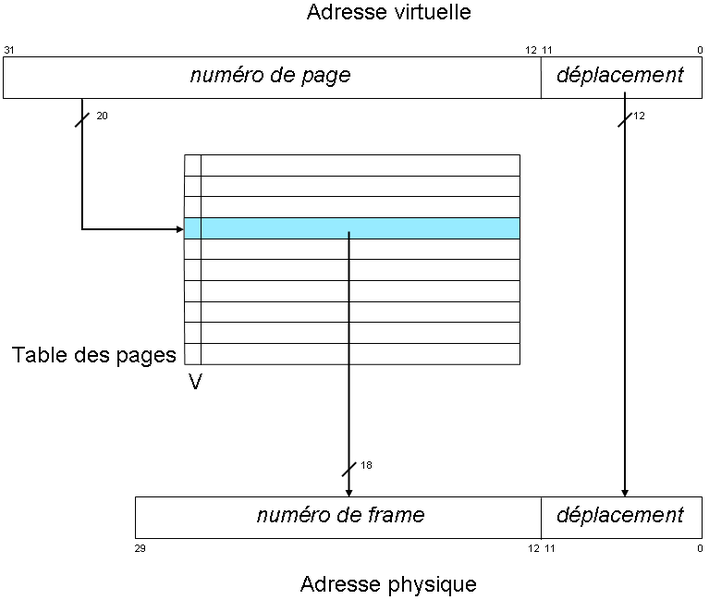
\includegraphics[scale=0.25]{tdp} \caption{Schéma de
        l'opération de traduction d'adresse par la table des pages}
        \label{fig:tdp}
    
    \end{figure}


  \subsection{Les threads}

    Les threads sont les fils d'éxécution du processus. On peut voir un
    processus comme une définition "statique" d'un programme, avec ses pages
    mémoire, les fichiers qu'il accède\ldots, tandis qu'un thread est une
    instance, actuellement en cours d'éxécution, de ce processus.
    
    Un thread est principalement défini par un \texttt{tid} (unique), un
    \texttt{pid} (le même que le processus auquel il appartient), une fonction à
    exécuter, les arguments relatifs à cette fonction, le processeur sur lequel
    il s'éxécute, son contexte d'éxécution et sa pile d'éxécution. L'espace
    d'adressage d'un thread est le même que celui du processus auquel il
    appartient, ce qui signifie que tous les threads d'un même processys
    partagent le même espace d' adressage, et donc que chacun peut voir les
    modifications des autres sur les variables communes. En revanche, les
    variables locales aux threads (celle des fonctions) seront mises dans la
    pile de ce dernier, et seront donc invisible aux autres\footnote{En théorie,
      chaque thread peut accéder aux piles des autres puisqu'ils sont dans le
      même espace d'adressage.  Néanmoins, cette opération est extrêmement
      compliquée puisqu'il faut être capable de trouver l'adresse de début de
    pile du thread que l'on veut "espionner".}.
    

  \section{L'appel système fork()} \label{sec:fork}

  \subsection{Rappels}

    Nous allons maintenant nous intéresser à ce qu'est un \texttt{fork()} dans
    un système UNIX. Avant de se plonger dans le code, il est important d'avoir
    un certain recul pour analyser cette fonction. On peut distinguer trois
    opérations de nature différente lors de cet appel:

    \begin{enumerate}[1-]

      \item[1-] allocation mémoire pour le processus fils que l'on va créer

      \item[2-] copie du père dans cette zone mémoire mémoire

      \item[3-] modification des quelques champs du processus fils (\texttt{pid,
        ppid, *parent}), etc\ldots

    \end{enumerate}

    Une fois ces étapes terminées, on a à l'adresse mémoire allouée à l'étape 1
    le nouveau processus, qui est une copie de son père, excepté les points
    suivants (liste non exhaustive pour l'instant): 

    \begin{enumerate}[1-]

      \item le \texttt{pid}

      \item le pointeur vers la struct \texttt{task\_s} représentant le parent

      \item la région virtuelle

      \item la région physique associée

    \end{enumerate}

    Bien que simple en apparence, cette opération est une des plus complexe sur
    un système UNIX. En effet, un processus est décrit par une multitude
    d'attributs, qui doivent tous êtres géré lors de ce dédoublement. Nous
    allons maintenant voir en détail comment fonctionne cette fonction, quels
    sont les structures de données impactées, et lesquels seront un problèmes
    pour nous.


  \subsection{Implémentation}

    Dans cette section, nous détaillerons le plus précisément possibles le
    fonctionnement de la fonction \texttt{fork()}. Les détails d'implémentations
    \textbf{spécifique à ALMOS}, bien que les principes fondamentaux restent les
    mêmes sur tout système UNIX.

    \subsubsection{La phase d'initialisation}

      Cette partie est très simple. Elle consiste à initialiser une structure
      \texttt{fork\_info\_t} (donnée en annexe) qui servira tout au long du
      \texttt{fork()}, sauvegarder le contexte d'exécution du processus père, et
      élire une paire $<cluster, cpu>$ pour le placement du
      thread\footnote{Actuellement, on se contente d'un placement par défaut. La
      DQDT\cite{almos-phd} est désactivée.}.
    

    \subsubsection{La phase de copie}

      Ici, on va allouer de la mémoire, copier toutes les informations partagées
      entre le père et le fils, et mettre les informations spécifiques du fils
      aux bons endroits.

      On va faire trois demandes de mémoire différentes \benumline \item
      \texttt{KMEM\_TASK} pour allouer les pages nécessaires pour stocker le
      nouveau processus (sa \texttt{struct task\_s}) \item \texttt{KMEM\_FDINFO}
      pour la structure contenant les descripteurs de fichiers ouverts
      \texttt{KMEM\_PAGE} pour la tables des pages. \todo{(demander plus de
      détails à Mohamed sur \texttt{task\_fd\_init()} parce que je suis pas sûr
      d'avoir tout compris)} \eenumline. Les deux informations les plus
      importantes sont \textbf{la table des descripteurs de fichiers ouverts} et
      \textbf{la table des pages}. En effet, les \texttt{struct vfs\_file\_s}
      pointées par les descripteurs de fichiers sont \textbf{partagées} par le
      père et le fils, et doivent par conséquent être cohérentes en permanence.
      Une autre structure partagée entre eux sont les régions virtuelles. Si le
      processus père a crée une région vituelle \textbf{partagée}, alors tout
      ses fils devront etre en mesure d'y accéder, tant en lecture qu'en
      écriture. Cette propriété est fondamentale pour la suite de notre exposé,
      et nous y reviendrons plus en détail dans la section~\ref{sec:problem}.

      Ensuite, on rempli le nouveau processus avec les informations qui lui sont
      spécifiques: son \texttt{pid}, le cluster où il va s'exécuter, le
      processeur sur lequel il va s'exécuter, son nombre de threads (\texttt{0}
      pour l'instant), son nombre de threads maximum son état
      (\texttt{TASK\_CREATE}), son nombre de fils, son nombre maximal de fils,
      et le binaire qu'il exécute. 

      On initialise le gestionnaire de signaux, et on place le processus dans le
      gestionnaire de tâches.

      Ensuite, on va commencer la copie depuis le processus père, via la
      fonction \texttt{task\_dup()}. On fait une demande d'allocation mémoire
      sur le cluster élu pour le placement, et on appelle cette fonction. Cette
      dernière va se charger de copier la table des descripteurs de fichiers
      ouverts dans celle que l'on a allouée juste avant.


    \subsubsection{L'allocation mémoire}

      Cette allocation se fait \textbf{sur le cluster élu}. En effet, la
      fonction \texttt{task\_dup()} récupère dans un premier temps le thread
      noyau du cluster élu, et c'est lui qui fera l'allocation mémoire. On
      demande dans un premier une région virtuelle \texttt{KMEM\_VM\_REGION},
      que l'on initialise à zéro. On met également l'arbre des régions à
      \texttt{NULL}. On demande ensuite une allocation de \textbf{pages
      physiques}. Une fois la page obtenue, on va copier le contenu la partie
      noyau de la table des pages du père dans le fils. Cette étape permet au
      processus fils de savoir ou sauter en cas d'appel système, et donc
      d'exécution de code noyau. Une fois cette étape terminée, on a
      correctement initialisé le processus fils depuis le père.  Il ne reste
      qu'à créer le premier \textbf{thread} pour ce processus.


    \subsubsection{Création du premier thread et début d'exécution}

      Cette opération est très simple et très rapide. On initialise une
      structure \texttt{thread\_s} via la fonction \texttt{thread\_dup()}, puis
      on place les bons flags sur le thread, on augmente le nombre de threads du
      processus, on passe son état à \texttt{READY}, on fait pointer le fils sur
      son père, et on ajoute son premier thread dans la liste des threads du
      processus créé plus haut (via \texttt{sched\_register()}. Enfin, on ajoute
      le nouveau processus dans la liste des fils du processus père.

      À ce moment là, on ressort de la fonction \texttt{sys\_fork()}, et un
      nouveau processus vient d'être crée, à partir de son père.

  \section{Problèmes} \label{sec:problem}

  À présent, nous allons voir quels sont les problèmes apportés par les choix
  architecturaux, tant matériels que logiciels.

  \subsection{Partage de structures}

    Comme nous l'avons vu en section~\ref{sec:fork}, un processus père partage
    avec son fils différentes structures. Les \texttt{struct vfs\_file\_s}
    (l'équivalent ALMOS des \texttt{struct file} de Linux) par exemple, mais
    aussi les régions virtuelles crées en mode \textbf{shared}, que l'on utilise
    dans les IPC~\cite{ipc}. Cette structure doivent se retrouver dans chaque
    fils crée depuis ce père, et doivent en permanence être cohérente entre tout
    ces processus. Chaque modification de l'un d'entre eux et visibles par les
    autres. Dans un contexte de machine non clusterisée, cette cohérence est
    implicite puisque la mémoire n'est pas découpée entre clusters. On profite
    ainsi de pouvoir accéder à n'importe quelle adresse mémoire (sauf les
    adresses noyau) depuis n'importe quel processus. La cohérence est donc
    intrinsèquement garantie, grâce au modèle architectural de la machine. Dans
    le cas de ALMOS, cette propriété n'est pas garantie.


  \subsection{Architecture clusterisée}

    On rappelle ici que l'architecture de travail est une architecture cc-NUMA
    clusterisée, et que ces derniers sont autonomes. Ils exécutent chacun le
    code noyau, chacun possédant sa pile d'exécution, ses données, et surtout
    son banc mémoire de 4Go. Ainsi, dans le cas d'une création à distance, il
    faudra répliquer les structures de données du père dans la mémoire du
    cluster où sera placée le fils. Cela nous amène à deux problèmes conséquents
    \benumline \item cette réplication aura un surcoût mémoire potentiellement
    important, du aux échanges de messages entre les clusters pour l'allocation
  de la mémoire et la copie des informations \item il faudra obligatoirement
    mettre en place un mécanisme de maintient de la cohérence entre ces deux
  structures représentant la même chose mais étant à deux endroits différents en
mémoire physique \item il faudra que ce mécanisme de cohérence passe à
  l'échelle, à minima, de l'architecutre TSA, puisque c'est cette dernière qui
  est considérée comme étant la plateforme de base pour exécuter
  ALMOS\eenumline.


  \subsection{}

  %\chapter{Principe de la solution envisagée}
\label{chap:sol}

  Notre solution est découpée en trois étapes incrémentales. Dans un premier
  temps, nous remettons en place le procédé de migration de processus
  mono-thread. Dans un second temps, nous ajoutons le support du
  multi-thread. Enfin, nous ré-implémentons un composant d'ALMOS appelé DQDT,
  nécessaire pour la politique de migration dans le noyau.

  \begin{paragraph}{Remarque:}
    Dans la section~\ref{sec:mono}, le mot \textit{processus} est utilisé pour
    désigner un processus composé d'un seul thread. Dans la suite de ce
    chapitre, à partir de la section~\ref{sec:multi}, on considère que les
    processus ont plusieurs threads.
  \end{paragraph}


  \section{Support des processus mono-thread}
  \label{sec:mono}

    Cette première étape a pour but de mettre en place deux mécanismes:
    \benumline \item la migration de processus entre noyaux \item la création
    distante de processus\eenumline. Pour compléter ces deux objectifs, il est
    nécessaire de définir l'ensemble des structures partagées par les processus
    et lesquelles doivent nécessairement être maintenues cohérentes tout au long
    de l'exécution.

    \subsection{Principes}

      \subsubsection{Rappels}

        L'appel système \texttt{fork()} est usuellement utilisé pour créer un
        processus dans un système. Lorsqu'un processus fait appel à cette
        fonction, un processus identique à l'appelant est créé. L'appelant est
        nommé \textit{père}, et le résultat est appelé \textit{fils}. Le fils
        étant une copie de son père, son exécution commence juste après l'appel
        système \texttt{fork()}.

        Pour qu'un fils exécute un autre programme que celui du père, il faut
        utiliser l'appel système \texttt{exec()}. C'est lui qui permet de
        remplacer le code exécuté par un processus.\\

        Dans la très grande majorité des cas, un appel à \texttt{fork()} est
        suivit d'un appel à \texttt{exec()}. C'est la principale manière de
        lancer des applications différentes dans un système\footnote{Voir
          \texttt{posix\_spawn()} pour une alternative.}. Un exemple
          d'utilisation de ces deux fonctions est donné par le
          Listing~\ref{lst:fork-exec}.

        \lstinputlisting[label={lst:fork-exec}, caption=Utilisation de
          \texttt{fork()/exec()}. La valeur de retour de \texttt{fork()} permet
          de différencier si le processus en cours d'exécution est le père ou le
          fils.]{include/code/example.c} \FloatBarrier

      \subsubsection{Migration}

        La migration de processus repose sur le mécanisme des RPC du
        noyau. Cette opération consiste à déplacer un processus dans un nouveau
        noyau pendant son exécution. Pour déplacer un processus, il faut envoyer
        les informations nécessaires au noyau destinataire afin qu'il puisse
        reconstruire l'espace virtuel du processus. On a notamment besoin des
        adresses de début et de fin:
        \begin{itemize}
          \item de la pile utilisateur
          \item du tas
          \item du code
          \item des arguments
          \item des données
        \end{itemize}
        Pour l'identification et l'exécution, il faut envoyer les informations
        suivantes:
        \begin{itemize}
          \item le \texttt{pid}
          \item l'identifiant du noyau d'origine
          \item le \texttt{pid} sur le noyau d'origine
          \item l'identificateur de groupe
          \item la priorité
          \item la politique d'ordonnancement\\
        \end{itemize}

        La migration n'est pas explicite pour le programmeur. Elle est à
        l'appréciation de la DQDT, présentée en section~\ref{sec:dqdt}. On veut
        simplement ici mettre en place un mécanisme via RPC permettant de migrer
        un processus à n'importe quel moment de son exécution.

      \subsubsection{Création distante}

        Migrer un processus pendant sa création, donc lors du \texttt{fork()},
        est une hypothèse que nous avons écartée. En effet, après avoir déplacé
        toutes les données du fils sur le nouveau noyau, la probabilité que ce
        dernier fasse un \texttt{exec()} est très grande. Par cet appel, il
        écrase toutes les données que l'on a déplacées juste avant. On paye donc
        le coût de la migration inutilement.\\

        Pour implémenter ce mécanisme, nous avons choisi de nous baser sur
        l'appel système \texttt{exec()}. Nous allons le modifier en ajoutant un
        appel aux fonctions de la DQDT. Si en retour le noyau s'aperçoit que le
        processus doit être migré, alors les informations citées précédemment
        seront envoyées. Ici, les données les plus importantes à transmettre
        sont le chemin vers l'exécutable et les arguments spécifiés dans l'appel
        \texttt{exec()} (voir l'algorithme~\ref{lst:fork-exec}). En effet, on
        veut que le processus qui sera créé exécute un nouveau code et pas celui
        de son père.\\

        Attendre un appel à \texttt{exec()} pour effectuer la migration permet
        de ne pas briser la localité spatiale des processus ayant un lien de
        parenté, et qui par définition accèdent aux mêmes données. On pense par
        exemple au navigateur web Firefox, qui gère ses onglets en utilisant un
        processus complet et non plus un thread~\citep{mozillaElectrolysis}.\\

        On note qu'un processus qui crée beaucoup de fils sans faire d'appel à
        \texttt{exec()} ne représente pas une menace pour la stabilité du
        système. En effet, au bout d'un temps $T$ borné, la DQDT verra la
        surchage engendrée par tous ces processus. Les mécanismes de migration
        expliqués précédemment seront alors activés.

        \begin{paragraph}{Remarque:}
          Un appel à \texttt{exec()} ne migre pas forcément un processus. La
          migration se fait selon la politique de la DQDT.
        \end{paragraph}


    \subsection{Maintien de cohérence}

      Comme nous l'avons vu précédemment, ces deux opérations représentent un
      enjeu quant aux structures de données que contiennent les processus, en
      particulier celles qu'ils partagent:
      \begin{itemize}
      \item les descripteurs de fichiers ouverts
      \item les zones mémoires partagées
      \end{itemize}

      Les descripteurs de fichiers contiennent des données qui doivent être
      maintenues cohérentes\footnote{C'est une obligation de la norme
        POSIX~\citep{posix2013} que le noyau ALMOS a choisi de respecter.}. Ces
      informations sont l'offset et le compteur de référence. Le premier indique
      la position à laquelle se trouve le processus dans un fichier. Le second
      permet de savoir combien de processus ont ouvert le même fichier.

      \begin{paragraph}{Remarque:}
        Cette cohérence s'applique également dans le cadre d'un processus ayant
        plusieurs threads : chaque action de l'un doit être visible des
        autres.\\
      \end{paragraph}

      Lorsqu'un processus ouvre un fichier puis crée un fils, les modifications
      du père doivent être visibles pour le fils, et inversement. Or, chaque
      modification déplace la tête de lecture. Afin de maintenir la cohérence
      dans le fichier, la valeur de l'offset doit être la même pour tous les
      processus ayant ouvert le fichier.

      Dans les sytèmes UNIX, chaque processus à son espace virtuel et ne peut
      pas accéder à celui des autres. Néanmoins, les noyaux permettent d'allouer
      de la mémoire en mode \texttt{SHARED}. Ainsi, deux processus peuvent se
      partager une certaine zone mémoire et ainsi échanger des
      informations. Pour des raisons évidentes, le contenu de ces zones mémoires
      doit impérativement être cohérent\footnote{On ne parle pas de la structure
        représentant la zone mémoire, qui elle est propre aux processus.}.


    \subsection{Accélération de la migration}

      Afin de faciliter le maintien de la cohérence et surtout d'accélérer la
      migration, nous devons redéfinir l'implémentation des descripteurs de
      fichiers et des zones mémoires. Il est nécessaire d'éliminer l'utilisation
      des pointeurs qui deviennent faux lorsqu'un processus change de noyau. En
      effet, une adresse dans un noyau $N$ n'est pas significative dans un noyau
      $N'$. Un exemple pour illustrer cela est celui des processus
      père/fils. Chaque processus doit savoir qui est son père, et possède un
      pointeur en direction de la \texttt{struct task} de ce dernier. Si le fils
      est migré sur un nouveau noyau, cette adresse n'est plus valable.

      Nous devons donc réduire au maximum le nombre de pointeurs, et notamment
      ceux utilisés pour gérer les descripteurs de fichiers ouverts ainsi que
      les zones de mémoire virtuelle d'un processus. Supprimer ces pointeurs
      implique de devoir changer l'implémentation de la structure de données
      utilisée pour stocker toutes les informations. Nous devons utiliser des
      tableaux pour enregistrer les informations sur les fichiers ouverts par
      les processus. Ces tableaux sont plus faciles à migrer puisqu'il s'agit
      simplement d'en faire une copie dans la mémoire du noyau destinataire.

      Nous avons actuellement deux solutions à l'étude:
      \begin{itemize}
        \item utiliser une table de hachage par calcul
        \item utiliser une table de hachage chainée
      \end{itemize}

      Aucune n'a pour l'instant été choisie. Néanmoins, quelque soit la solution
      envisagée, les entrées et sorties sont similaires, ce qui nous permet de
      n'effectuer qu'une seule spécification. Nous allons utiliser l'adresse
      virtuelle accédée comme entrée de la fonction de hash. En sortie, nous
      obtenons l'adresse physique de la région virtuelle associée.

      \begin{center}
        \texttt{hash(v\_addr) = v\_reg\_addr}
      \end{center}

      La première solution nous garantie de n'avoir qu'une table à
      gérer. Néanmoins, cette gestion est assez difficile à implémenter. À
      l'inverse, la table de hash chainée est plus simple à mettre en \oe uvre
      mais les indirections que nous pensons utiliser en feront un objet plus
      complexe que la précédente solution. Ces deux possibilités n'ont pour
      l'instant pas été estimées en terme de coût pour le système. Elles restent
      donc à l'état d'hypothèse jusqu'à ce que l'une d'elle s'avère plus
      efficace.


  \section{Ajout du multi-thread}
  \label{sec:multi}  

    Une fois le support des processus mono-thread en place, nous devons ajouter
    le support du multi-thread. Cette opération s'avère très délicate, et
    représente probablement l'étape la plus compliquée de ce stage.\\

    Dans la section~\ref{sec:mono}, nous avons parlé des structures de données
    critiques pour les processus mono-thread. Nous allons à présent nous
    intéresser aux processus multi-thread. Après étude du problème, nous avons
    principalement deux structures qui posent problème (en plus de celle vues en
    ~\ref{sec:mono}):
    \begin{itemize}
      \item la table des pages
      \item les signaux
    \end{itemize}  

    \subsection{La table des pages}

      La table des pages est la structure de données des processus permettant
      les traductions des adresses virtuelles en adresses physiques. Chaque
      processus possède sa propre table des pages, et tous les threads d'un
      processus accèdent à cette table.

      Le problème de cette structure sont les accès fréquents lors des miss TLB
      (le cache de traduction d'adresses virtuelles $\leftrightarrow$
      physiques). Si l'on migre un thread du processus sur un autre noyau, ce
      dernier accèdera par passage de messages à la table, ce qui n'est pas
      envisageable pour des raisons de performances. Il faut donc copier la
      table des pages entièrement, ce qui n'est pas gratuit, et maintenir
      ensuite une cohérence entre toutes les tables répliquées dans les
      clusters. En prenant en compte le fait que chaque processus possède une
      table de page, les surcoûts liés aux communications apparaîssent
      rapidement.

      Pour répondre à cette problématique, nous allons intégrer le concept des
      processus hybrides~\citep{almaless2014universite}. Un processus hybride
      contient des threads qui ont leur propre espace virtuel qui n'est plus
      accessible par les autres threads du processus. Le noyau maintient
      néanmoins la cohérence entre ces espaces. De plus, chaque thread possède
      sa table des pages, qui contient des pages communes avec les autres
      threads du processus, mais également ses propres pages locales. Le
      mécanisme proposé est illustré par la figure~\ref{fig:almos-page-table}.

      \begin{figure}[ht]
        \centering
        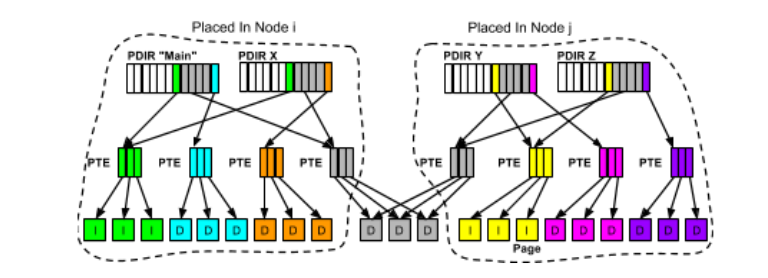
\includegraphics[width=\textwidth]{almos-page-table}
        \caption{Organisation de la table des pages pour quatre threads d'un
          même processus. Deux threads sont placés sur un cluster $i$, et deux
          sur un cluster $j$. Les threads partagent certaines pages de données
          et d'instructions, parfois entre clusters, mais ont également leurs
          pages privées~\citep{almaless2014universite}.}
        \label{fig:almos-page-table}
      \end{figure}

      L'intérêt des processus hybrides est double:

      \begin{itemize}
        \item on évite le goulot d'étranglement sur la table des pages
        \item les espaces virtuels des threads ne sont plus stockés dans le
          processus mais sont indépendants, on a donc économisé de la place dans
          la mémoire virtuelle du processus
      \end{itemize}

      Cette solution permet de minimiser le coût de la cohérence des tables
      entre tous les réplicas et permet également d'alléger les accès
      atomiques. En effet, une application massivement parallèle minimisera les
      dépendances de données entres threads, et donc les pages communes.\\

      Par manque de temps, ce concept n'a pas été implémenté dans le noyau
      ALMOS. Nous allons donc devoir le mettre en place, avec dans un premier
      temps l'objectif d'avoir une table des pages distribuée entre les
      threads.


    \subsection{Les signaux}

      Dans cette partie, nous allons devoir mettre en place des mécanismes pour
      la transmission des signaux lorsque les threads sont distribués sur
      plusieurs noyaux. En effet, la norme POSIX stipule que la portée des
      signaux est un processus dans son ensemble~\citep{man2015signal}.

      Pour cela, il faudra redéfinir la notion de \texttt{pid}. Un \texttt{pid}
      sera découpé en deux parties \benumline \item la partie haute indiquera la
      valeur du cluster sur lequel s'exécute le thread \item la partie basse
      donnera la valeur classique du \texttt{pid} sur ce
      cluster\eenumline. L'application d'un masque sur le champ \texttt{pid}
      permettra alors d'obtenir l'information souhaitée.

      Enfin, après une migration, un processus enverra sa nouvelle adresse au
      noyau d'origine, qui le modifiera dans sa table des processus. Ainsi, le
      noyau d'origine des processus connait en permanence la localisation de ses
      fils sur la machine. Ce mécanisme nous permet de pouvoir transmettre les
      signaux.


  \section{La DQDT}
  \label{sec:dqdt}

    Cette partie du stage est ``optionnelle''. La ré-implémentation de ce
    composant est un besoin réel pour ALMOS, néanmoins cela implique que les
    étapes présentées précédemment soient finalisées.

    La DQDT, pour \textit{Distributed Quaternary Decision Tree}, est le
    composant d'ALMOS assurant une vision cohérente et temps-réel\footnote{C'est
      un abus de langage qui est fait ici. Nous voulons simplement montrer que
      la DQDT permet d'avoir en permanence les taux d'utilisation des 4096
      processeurs de la plateforme.} de l'utilisation des ressources. Dans la
    version de Ghassan~\citet{almaless2014universite}, la DQDT repose sur des
    serveurs répliqués dans tous les clusters. Chaque cluster physique
    représente une feuille de la DQDT. Ces serveurs récupèrent les informations
    sur l'occupation de la machine (c\oe urs et mémoire), et calculent une
    moyenne d'utilisation pour chaque cluster. Cette information est stockée
    dans un n\oe ud de l'arbre. Chaque étage de l'arbre représente un niveau
    d'abstraction. Comme le montre la figure~\ref{fig:dqdt-logical}, le premier
    niveau, en noir, est celui des clusters physiques. Le second niveau, en
    bleu, regroupe 4 clusters. C'est un cluster logique de niveau 1. Le dernier,
    en rouge, regroupe quatre clusters logiques de niveau 1 dans un cluster
    logique de niveau 2. Ces niveaux sont matérialisés par les étages de
    l'arbre, comme le montre la figure~\ref{fig:dqdt-tree}.\\

    \begin{figure}[ht]
      \begin{subfigure}[b]{0.5\textwidth}
        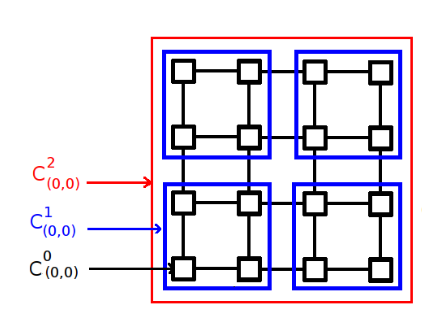
\includegraphics[scale=0.4]{dqdt-logical}
        \caption{Découpage de la plateforme}
        \label{fig:dqdt-logical}
      \end{subfigure}
      \begin{subfigure}[b]{0.4\textwidth}
        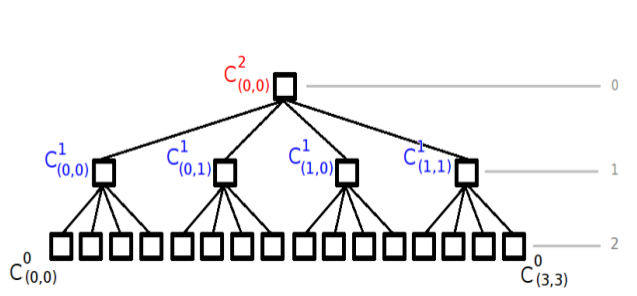
\includegraphics[scale=0.4]{dqdt-tree}
        \caption{Représentation du découpage}
        \label{fig:dqdt-tree}
      \end{subfigure}
      \caption{Construction de la DQDT~\citep{almaless2014universite}.}
    \end{figure}

    La DQDT, comme la plupart des composants noyaux d'ALMOS, repose sur le
    mécanisme de la mémoire virtuelle répartie entre les clusters. Si l'on
    change ALMOS en multi-noyau, les serveurs de la DQDT ne peuvent plus
    communiquer grâce à la mémoire virtuelle. Ils sont obligés d'utiliser le
    passage de messages entre les noyaux.

    Notre but est de changer le schéma de communication de la DQDT. Deux
    techniques peuvent être utilisées:
    \begin{itemize}
      \item avoir une solution portable sur n'importe quelle architecture
        matérielle : nous utilisons le passage de messages
      \item avoir une solution efficace sur l'architecture TSAR : nous profitons
        de mécanismes matériels nous permettant d'accéder directement à la
        mémoire physique des clusters voisins.
    \end{itemize}

    Nous allons dans un premier temps implémenter une version efficace sur TSAR,
    puis selon le temps restant, une solution générique.


    \nomenclature{DQDT}{Distributed Quaternary Decision Tree}
    \nomenclature{RPC}{Remote Procedure Call}
    \nomenclature{UNIX}{Uniplexed Information and Computing Service}
    \nomenclature{PDIR}{Page DIRectory}
    \nomenclature{PTE}{Page Table Entry}

  \begin{thebibliography}{1}

  \bibitem{almos-cfse} Ghassan Almaless. \emph{ALMOS : un système d'exploitation
    pour manycores en mémoire partagée cohérente}. \relax In Proceedings of the
    8th French conference on Operating Systems (CFSE), the French chapter of
    ACM-SIGOPS, GDR ARP, Saint-Malo, France, 2011.

  \bibitem{almos-phd} Ghassan Almaless. \emph{Operating System Design and
    Implementation for Single-Chip cc-NUMA Many-Core}. \relax Ph.D thesis, UPMC,
    France, 2014.

  \bibitem{posix} \emph{The POSIX standard} available at
    \url{http://www.opengroup.org/austin/}

  \bibitem{tsar}{\emph{The TSAR Project} available at \relax
    \url{https://www-asim.lip6.fr/trac/tsar}}

\end{thebibliography}

  \newpage
  \section*{Annexes}

  \subsection*{La structure task\_s}
  
    \lstinputlisting[firstline=47, lastline=97, style=almos,
      caption=\texttt{struct task}.Cette structure représente la notion la plus
      haut-niveau possible pour le système d'exploitation: les tâches qu'il doit
      ordonnancer. Chaque tâche est un ensemble de structure permettant de la
      définir.On trouve principalement tout ce qui concerne les zones mémoire de
      la tâche  sa localisation sur la machine (en terme de numéro de cluster et
      de cpu) et tout ce qui conserne les fichiers tout les threads de cette
    tâche. Lors d'un \texttt{fork()} c'est cette structure qui est dupliquée
  puis modifiée.]{include/code/task.h} \label{lst:task}
    
  \subsection*{La structure fork\_info}

  \lstinputlisting[style=almos, firstline=47, lastline=56,
  caption=\texttt{struct fork\_info\_t}. \label{lst:fork_info_t} Cette structure
est utilisée tout au long du fork pour passer les informations vitales entre
toutes les fonctions.]{include/code/task.c}
    
    \newpage

  \subsection*{Le VFS}

    \subsubsection*{La structure node}

      \lstinputlisting[style=almos, firstline=78, lastline=103,
      caption=\texttt{struct vfs\_node\_s}.]{include/code/vfs.h}
      \label{lst:vfs_node}
  
    \subsubsection*{La structure file}
   
      \lstinputlisting[style=almos, firstline=105, lastline=117,
      caption=\texttt{struct vfs\_file\_s}.]{include/code/vfs.h}
      \label{lst:vfs_file}
  
      %Cette structure est l'équivalent de la \texttt{struct file} du noyau
      %Linux.  Ce niveau d'abstraction permet quant à lui de représenter la
      %manipulation de l'information: \texttt{read(), write()}, les offsets des
      %têtes de lecture\ldots

 

\end{document}
